\documentclass{report}

\usepackage{subcaption} % package for subfigures
\usepackage{hyperref}  % package for linking figures etc
\usepackage{enumitem}  % package for description with bullets
\usepackage{graphicx}  % package for importing images
\usepackage{mathtools} % package for math equation
\usepackage{mathrsfs}  % package for math font
\usepackage{indentfirst} % package for getting ident after section or paragraph
\usepackage[export]{adjustbox}
% \usepackage{amsmath}

\setlength{\parindent}{2em} % how much indent to use when we start a paragraph

\graphicspath{ {./theory/figures/} }       % path for images

\begin{document}

\chapter{Classification stage}
\section{Description}
After getting all proposed tubes, it's time to do classification. As classifiers we use several approaches includingn
a Recursive Neural Network (RNN) Classifier, a Support Vector Machine (SVM) Classifier and a Multilayer perceptron (MLP).
\\
\textbf{Pending Change the sxima...}
\\
\begin{figure}[h]
  % 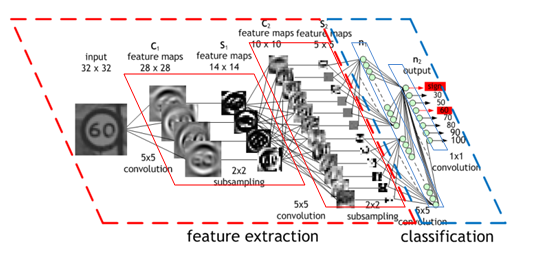
\includegraphics[scale=0.7]{convolutional_neural_network_structure} \]
  \centering
  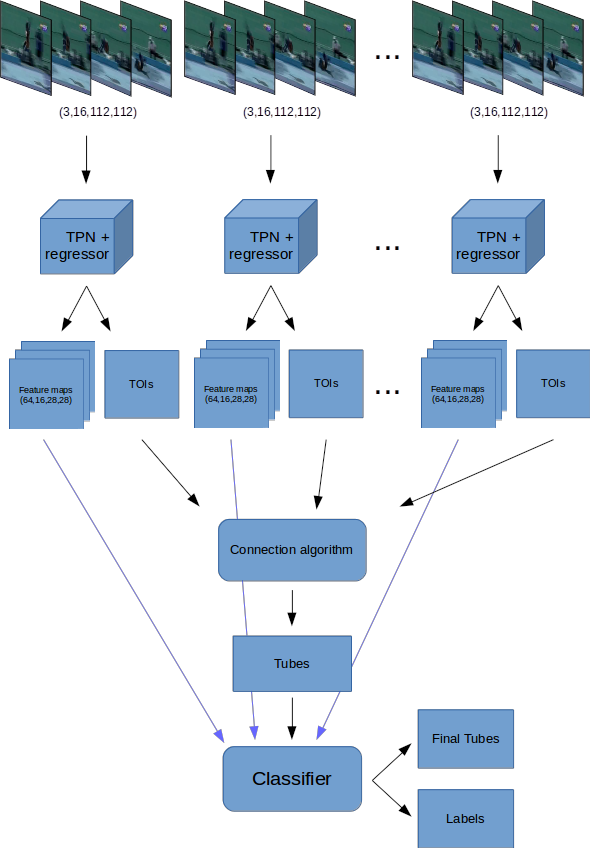
\includegraphics[scale=0.7]{model}
  \caption{Structure of the whole network}
  \label{fig:whole_network}
\end{figure}

The whole procedure of classification is consisted from the following steps:
\begin{enumerate}
\item Seperate video into small video clips. Feed TPN network those video clips and get as output
  150 ToIs and their corresponding features for each video clip.
\item Connect the proposed ToIs in order to get video tubes which may contain an action.
\item For each candidate video tube, which is a sequence of ToIs, feed it into the classifier
  for verification.
\end{enumerate}

The general structure of the whole network is depicted in figure \ref{fig:whole_network}, in which blue arrows show that
features go straight up to the classifier. (Pending... Change that)


\section{Preparing data for classification - Linear and RNN Classifiers}

(Pending... Introduction about Linear and RNN classifiers)
(Pending.. also an image of Linear classifier)

  

In order to train our classifier, we have to execute the previous steps for each video. However, each video
has different number of frames and reserves too much memory in the GPU. In order to deal with this situation
we give as input one video per GPU. So we can handle 4 videos simultaneously. This means that a regular
training session takes too much time for just 1 epoch. \par
The solution which we came with, is to precompute the features for both positive video tubes and negative video tubes.
Then we feed those features to our classifier and we train it in order to disciminate their classes.
Again, we mainly experiment with jHMDB dataset because it has smaller number of videos than UCF dataset, so this means
less memory usage for saving the features.\par
At first, we extract only groundtruth video tubes' features and the double number of background video tubes. We chose this
ratio between positive and negative tubes inspired by \cite{jjfaster2rcnn}, in which it has 0.25 ratio between foreground
and background rois and chooses 128 roi in total. Respectively, we chose a little bigger ratio because we have only 1 groundtruth
video tube in each video. So, for each video we got 3 video tubes in total.
\textbf{(Pending describe extracting procedure)}
Also, we extracted the validation video tubes in order to do a first assesment in our classifiers's performance in ideal conditions. 

Then, after extracting those features, we trained both linear and RNN classifiers. The Linear classifier needs a fixed input size,
so we used a pooling function in the dimension of the videos. So, at first we had a feature map of 3,512,16 dimensions and then we
get as output a feature maps of 512,16 dimensions. We used both max and mean pooling as show in the results below. For the RNN
classifier, we do not use any pooling function before feeding it. For both classifiers, at first, we didn't considered a fixed
threshold for confidence score.
(Pending results in Linear... Table)

The results are disappointing.
As we can see in the table, RNN classifier cannot classify very well because, probably, the duration of the videos are so small
so we stopped using it in jHMDB dataset. In the Linear classifier, we noticed that every tube is considered as background tube.
That means that Linear classifier gets overfitted with trained data and cannot handle unknown data. So, we thought that we
need a classifier which can \"learn\" very easily, with little data. So we chose to try a support vector machine classifier

\section{Support Vector Machine (SVM)}
\subsection{First steps}
SVMs are classifiers defined by a separating hyperplane between trained data in a N-dimensional space. The main advantage of using a SVM
is that can get very good classification results whenwe have few data available.
\textbf{write more introduction and a pic, Pending...}
The use of SVM is inspired from \cite{Girshick:2015:FR:2919332.2920125}. \par
SVM is trained using hard negatives. This means that we have 1 classifier for each class which has only 2 labels, positive and negative.
As positive we have tubes that contains the groundtruth action and as negative we can have  groundtruth action tubes from other classes,
background tubes or a combination of them.

Pending....

\subsection{Temporal pooling}
After getting first results, we implement a temporal pooling function inspired from \cite{DBLP:journals/corr/HouCS17}. We need a
fixed input size for the SVM. However, our tubes' temporal stride varies from 2 to 5. So we use as fixed temporal pooling equal
with 2. As pooling function we use 3D max pooling, one for each filter of the feature map.  So for example, for an action tube
with 4 consecutive ToIs, we  have 4,256,8,7,7 as feature size. We seperate the feature map into 2 groups using \textit{linspace}
function and we reshape the feature map into 256,k,8,7,7 where k is the size of each group, After using 3D max pooling, we get
a feature map 256,8,7,7 so finally we concat them and get 2,256,8,7,7.

After temporal pooling, we feed again our SVM and we in the following results.

Pending...

\subsection{Adding more groundtruth tubes}
From above results, we notice that SVM cannot get very good results, too. So, we thought that we should try to add more positive
examples in our training procedure. 

\section{MultiLayer Perceptron (MLP)}
Last but not least approach is a Multilayer perceptorn (MLP). More specifically, we extract the 3 last residulal layers of 3D ResNet34
and we add a classification layer.  
\subsection{Extract features}
\subsection{Regular training}

\section{Final Improvements}
After classification, we relize that a lot of classified tubes overlap and represent the same action. So, we use again NMS algorithm in order
to remove unnecessary tubes. The new model can be seen in figure \ref{fig:network_nms}.

\begin{figure}[h]
  % 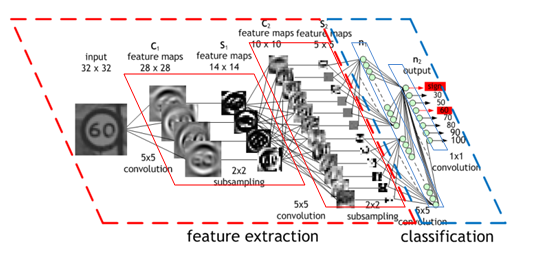
\includegraphics[scale=0.7]{convolutional_neural_network_structure} \]
  \centering
  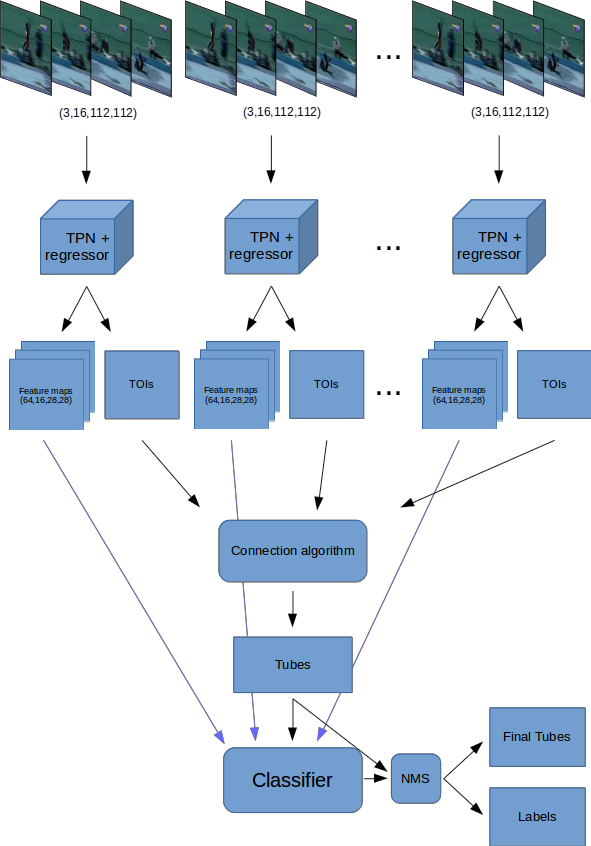
\includegraphics[scale=0.7]{model_nms}
  \caption{Structure of the network with NMS}
  \label{fig:network_nms}
\end{figure}

\end{document}
